
\subsection{Results and interpretation}

    Under the main tempered prior, independent OU multi-time coverage is
    0.8056, with interval score 10.092
    and finite-mean forecast RMSE 2.406.
    Shared OU coverage is 0.9722, with interval score
    9.449 and RMSE 2.191.
    Mean observed-minus-mean-forecast bias remains
    1.642 and 1.370, respectively.
    These results address the moment pathology while retaining the late
    underprediction as a separate model-adequacy issue.

    The historical finite-subset independent and shared OU interval scores
    were 10.164 and
    9.371; their coverages were
    0.8056 and
    0.9722. Those earlier mean-based quantities
    remain finite-subset diagnostics. The new predictive means have a
    mathematically finite target under the new priors. This does not make
    small differences in retrospective scores statistically decisive.

    At the 15 distinct one-step targets, independent and shared OU coverages
    are 0.8667 and
    0.9333. Their mean-forecast RMSE values are
    1.926 and
    1.623; median-forecast RMSE values are
    1.945 and
    1.654.
    Joint density scores retain the modeled dependence between trial
    responses. Table~\ref{tab:tempered-one-step} reports all four models;
    Table~\ref{tab:tempered-rollout} retains both prespecified tail strengths.

    All 40 cases meet the computation gates. The largest monitored
    $\widehat R$ is 1.0059, minimum bulk ESS
    929, and minimum tail ESS
    423. The minimum raw ESS for monitored
    conditional-response-mean observables is
    948; their largest estimated MCSE
    is 0.0717 response units. Those
    functional diagnostics use every eighth retained draw. New fits retain
    36000 to 108000
    draws per chain after 6000 warmup iterations. They support a finite-run
    computation check, not a proof of convergence or predictive calibration.

    For the two main-prior OU models at cutoff 132, posterior integration
    using 6000, 12000, and 24000 components shifts means by at most
    0.014 response units and interval
    endpoints by at most 0.015
    relative to the 6000-component result. These are numerical sensitivity
    checks, distinct from the analytic moment bound.

    No discrepancy model or tail strength is promoted to the mechanistic
    reference. Prior medians are matched, but prior shapes and upper
    quantiles change. Only two fixed tail strengths were tested here;
    the earlier half/double noise-median sensitivity is not a sensitivity
    analysis of this new family. The proposed prospective protocol retains
    its earlier priors and median point forecast until explicitly amended.
    Unconfirmed physical units, experimental dependence, and unavailable
    independent trajectories remain unresolved. A finite predictive mean
    resolves REV-11's mathematical concern for this new family, while
    REV-07's predictive adequacy and REV-10's experimental validation remain open.

\begin{figure}[htbp]
    \centering
    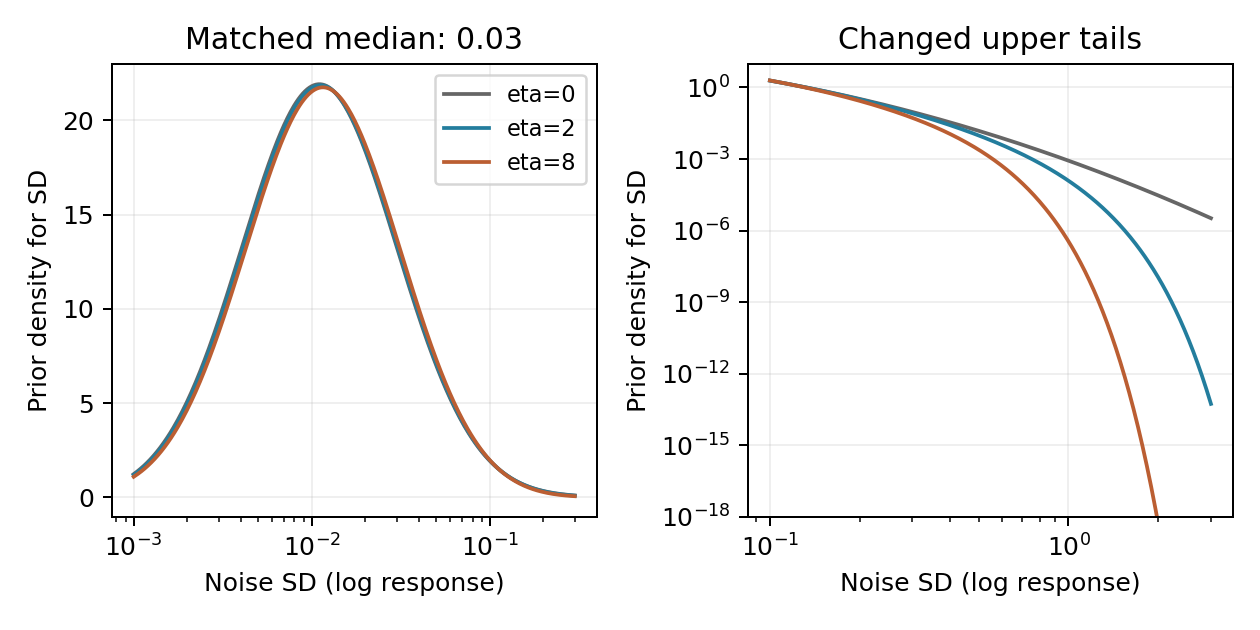
\includegraphics[width=\textwidth]{../results/tempered/noise_prior_comparison.png}
    \caption{Noise-SD prior densities with matched median 0.03. The stronger
    upper-tail penalties change the 95th percentiles and tail integrability;
    they impose no finite upper SD bound. Both latent and measurement SDs
    receive the same separate prior.}
    \label{fig:tempered-priors}
\end{figure}
\begin{figure}[htbp]
    \centering
    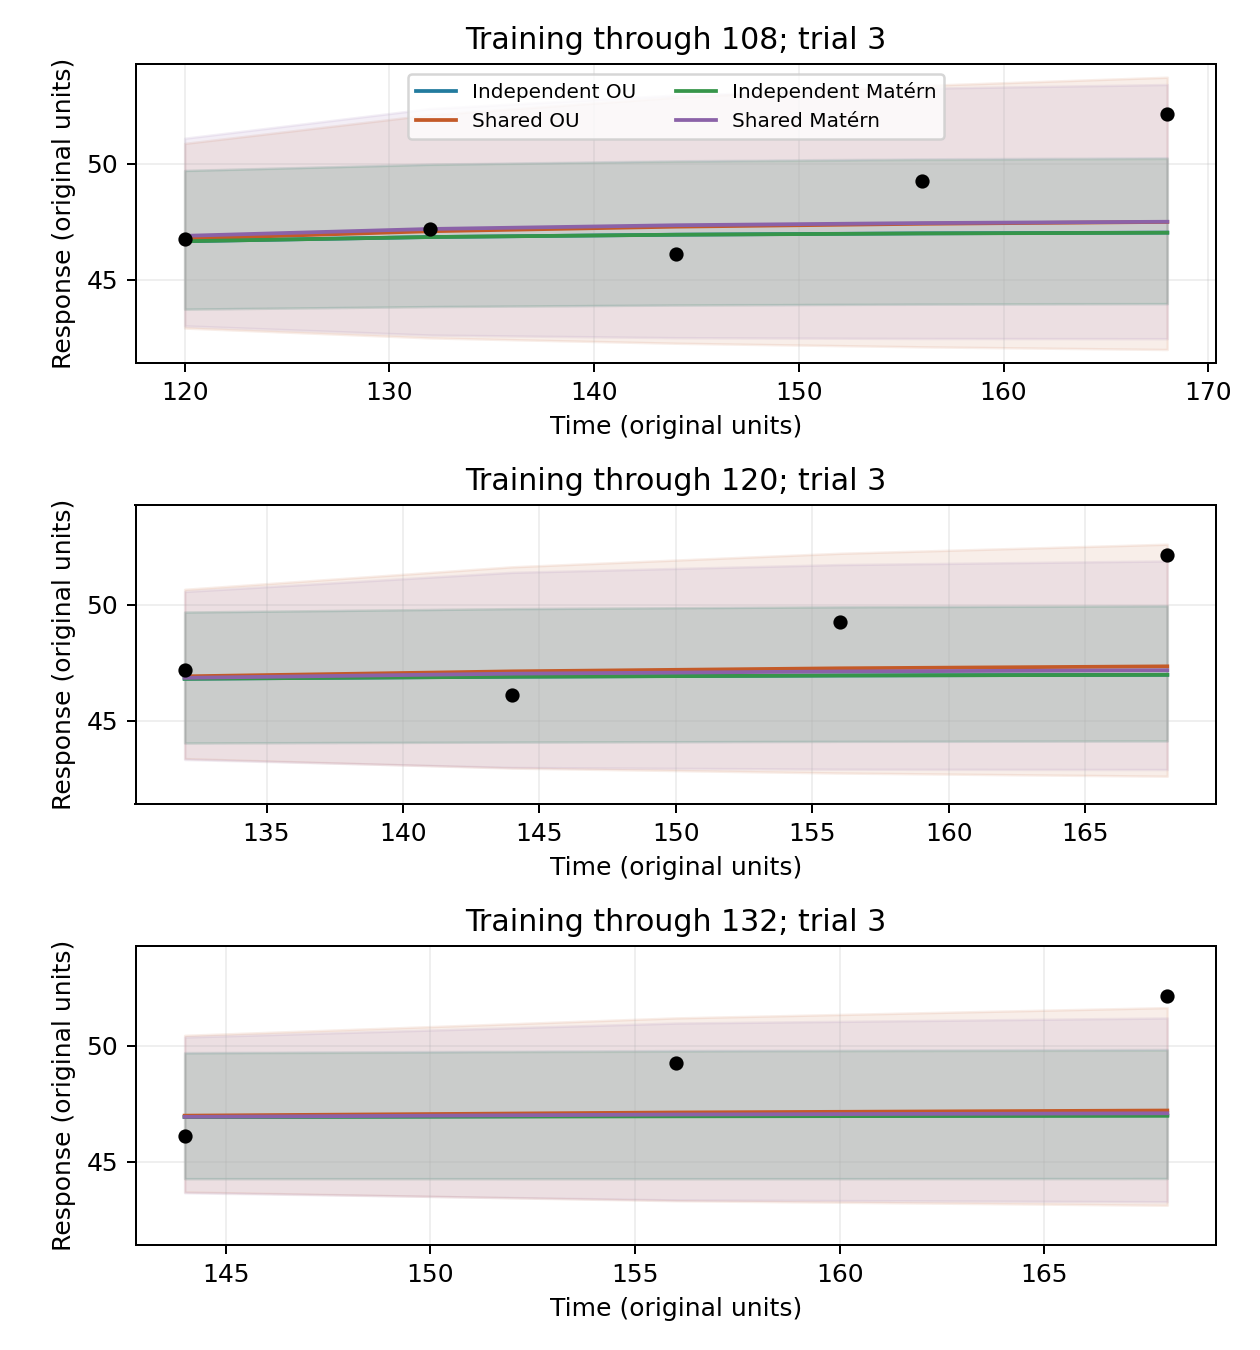
\includegraphics[width=\textwidth]{../results/tempered/forecast_comparison.png}
    \caption{Main tempered prior: trial 3 predictive means and central
    90 percent observation intervals. Black points are held-out responses.
    All reported metrics use the three trial series. These means estimate
    finite response expectations under the new model.}
    \label{fig:tempered-forecast}
\end{figure}
